% Template for Cogsci submission with R Markdown

% Stuff changed from original Markdown PLOS Template
\documentclass[10pt, letterpaper]{article}

\usepackage{cogsci}
\usepackage{pslatex}
\usepackage{float}
\usepackage{caption}

% amsmath package, useful for mathematical formulas
\usepackage{amsmath}

% amssymb package, useful for mathematical symbols
\usepackage{amssymb}

% hyperref package, useful for hyperlinks
\usepackage{hyperref}

% graphicx package, useful for including eps and pdf graphics
% include graphics with the command \includegraphics
\usepackage{graphicx}

% Sweave(-like)
\usepackage{fancyvrb}
\DefineVerbatimEnvironment{Sinput}{Verbatim}{fontshape=sl}
\DefineVerbatimEnvironment{Soutput}{Verbatim}{}
\DefineVerbatimEnvironment{Scode}{Verbatim}{fontshape=sl}
\newenvironment{Schunk}{}{}
\DefineVerbatimEnvironment{Code}{Verbatim}{}
\DefineVerbatimEnvironment{CodeInput}{Verbatim}{fontshape=sl}
\DefineVerbatimEnvironment{CodeOutput}{Verbatim}{}
\newenvironment{CodeChunk}{}{}

% cite package, to clean up citations in the main text. Do not remove.
\usepackage{apacite}

% KM added 1/4/18 to allow control of blind submission
\cogscifinalcopy

\usepackage{color}

% Use doublespacing - comment out for single spacing
%\usepackage{setspace}
%\doublespacing


% % Text layout
% \topmargin 0.0cm
% \oddsidemargin 0.5cm
% \evensidemargin 0.5cm
% \textwidth 16cm
% \textheight 21cm

\title{Title TBD}


\author{Kennedy Casey \\
        University of Chicago \\
        \texttt{\small{kbcasey@uchicago.edu}}
\And \textbf{Mary Elliott} \\
             University of Texas at Dallas \\
             \texttt{\small{maryle18@gmail.com}}
\And \textbf{Anapaula Silva Mandujano} \\
             University of Chicago \\
             \texttt{\small{anapaula@uchicago.edu}}   
\And \textbf{Kimberly Shorter} \\
             University of Chicago \\
             \texttt{\small{klshorter@uchicago.edu}}
\AND \textbf{Elizabeth Mickiewicz} \\
             University of Chicago \\
             \texttt{\small{lizmick9@uchicago.edu}}         
\And \textbf{Mara Duquette} \\
             University of Chicago \\
             \texttt{\small{duquettemara@uchicago.edu}}
\And \textbf{Elika Bergelson} \\
             Duke University \\
             \texttt{\small{elika.bergelson@duke.edu}}
\And \textbf{Marisa Casillas} \\
             University of Chicago \\
             \texttt{\small{mcasillas@uchicago.edu}}}

\newlength{\cslhangindent}
\setlength{\cslhangindent}{1.5em}
\newenvironment{CSLReferences}%
  {}%
  {\par}

\begin{document}

\maketitle

\begin{abstract}


\textbf{Keywords:}

\end{abstract}

\hypertarget{introduction}{%
\section{Introduction}\label{introduction}}

The artifacts of everyday life reflect our routines, aspirations,
relationships, and more. In particular, the objects that we regularly
pick up and handle---a coffee cup, a laptop, a baby bottle---offer a
window into the physical, social, and cultural contexts that shape our
understanding of the world. In this paper, we take a glimpse into
everyday life at its beginnings by exploring children's at-home object
handling from early infancy until age four. We contextualize our study
with respect to the effects of object-centric interaction on word
learning, though we note that different analyses of these same data
could shed new light on other types of social learning as well as motor
development (see Herzberg, Fletcher, Schatz, \& Tamis-LeMonda, 2021 on
the latter point).

\hypertarget{object-handling-and-word-learning}{%
\subsection{Object handling and word
learning}\label{object-handling-and-word-learning}}

For young learners, objects---along with their associated activities and
surrounding language---form a critical source of input for word
learning. Hands (and what they are handling) can be reliable indicators
of what someone is doing and talking about during object play ,
facilitating children's ability to map word forms onto their meanings in
and across real-time interaction (e.g., Yu \& Smith, 2013; Yurovsky,
Smith, \& Yu, 2013). Present, attended-to objects also influence the
babble of children who have acquired stable consonants (Laing \&
Bergelson, 2020). Further, caregivers' tendency to use nouns referring
to objects in the here-and-now positively predicts their children's
early word comprehension (Bergelson \& Aslin, 2017).

How frequently do children engage in object-centric interactions? First,
hands---others' and their own---are in good supply in young children's
view of the world, especially after early infancy (Fausey, Jayaraman, \&
Smith, 2016; Jayaraman, Fausey, \& Smith, 2017; Long, Kachergis,
Agrawal, \& Frank, 2020), topping out at visible presence \(\sim\) 30\%
of the time. Infants' own object handling is also relatively frequent:
Herzberg and colleagues (2021) find that US infants handle objects
\(\sim\) 60\% of the time during at-home play, Yu and colleagues (2013)
find \(\sim\) 70\% when including joint handling with adults in US
in-lab object play, and Casillas \& Elliott (2021) find \(\sim\) 15 and
17\% object handling in daylong photo streams in a Papuan and a Mayan
community, respectively. Note, however, that \emph{labeling} of
object-relevant features (e.g., names and associated concepts) is the
critical second ingredient for word learning, which may only occur
during a small subset of total object handling time. Additionally, the
likelihood of talk about objects that are being handled in the here and
now---a flagship feature of contingent caregiver talk (e.g., McGillion
et al., 2013)---fluctuates across high and low activity periods of
interaction (Bergelson, Amatuni, Dailey, Koorathota, \& Tor, 2019).

Overall, while prior work makes a strong case for the impact of
children's object-centric interactions on their word learning, the
findings: (a) are limited to a culturally narrow sample of populations,
(b) have tended to rely on short recordings that limit the scope of
object-centered interactions analyzed, and (c) have rarely examined in
detail the distributions of individual objects that children typically
interact with at home (exceptions include Bergelson, Amatuni, Dailey,
Koorathota, \& Tor, 2019; Casillas \& Elliott, 2021; Herzberg, Fletcher,
Schatz, \& Tamis-LeMonda, 2021).

\hypertarget{object-handling-across-age-and-culture}{%
\subsection{Object handling across age and
culture}\label{object-handling-across-age-and-culture}}

Children's object handling input changes enormously across the first few
years due to both maturational constraints and culture-specific
caregiving practices. In early infancy, children have little ability to
hold things or to control their posture, primarily experiencing objects
through what others bring near to them. Faces, rather than objects, may
make up a much greater proportion of their social input early on
(Fausey, Jayaraman, \& Smith, 2016; Jayaraman, Fausey, \& Smith, 2017;
but see also Long, Kachergis, Agrawal, \& Frank, 2020). However, later
gains in manual dexterity and gross motor skill (e.g., sitting,
crawling, walking) increasingly widen children's ability to seek, reach,
and grab a diversity of objects in their environment. Increasing motor
development not only gives children greater control over what objects
handle but also how they elicit social information relating to objects
and for how long object-centered interactions last (Adolph, Karasik, \&
Tamis-LeMonda, 2010; Gaskins, 2000; Herzberg, Fletcher, Schatz, \&
Tamis-LeMonda, 2021; Kretch, Franchak, \& Adolph, 2014; Sanchez, Long,
Kraus, \& Frank, 2018).

Early access to objects is also shaped by culture-specific practices for
carrying children, keeping them safe and warm, and scaffolding the
development of locally valued capacities (e.g., word learning in many US
families, walking in Kenyan Kipsigis families: Super, 1976; see Adolph,
Karasik, \& Tamis-LeMonda, 2010, for an overview). The array of objects
available to children will also vary in type and prevalence
cross-culturally. Objects spread via globalization (e.g., plastic bags)
and objects with a basic functional role that has arisen similarly
across many groups (e.g., spoon-like things for eating) are likely to
appear in widely, while other objects remain specific to people and
places (e.g., the gourd and bombilla for drinking mate in much of South
America, stemming from Indigenous Guaraní and Tupí tradition). Take, for
example, middle-class US family homes, which have been noted for their
large quantities of possessions (``clutter''), much of which is designed
specifically for children (e.g., toys and books, Arnold, Graesch, Ochs,
\& Ragazzini, 2012). We might infer, based on this distribution, that
much of what children do and talk about at home is tailored to what
particularly interests them. Thus, children's worlds, in this sense,
look very different from their caregivers'. Recent work by Herzberg and
colleagues (2021) underscores this point with infancy data; 13- to
23-month-olds spent nearly 70\% of their time in object play with toys
or a mix of toys and non-toys, with \(\sim\) 100\% of infants playing
with children's books and stuffed animals, and a total of 32 toy types
appearing in \(\ge\) 25\% of infants' play. Non-toy play was also
common, but still appeared to predominantly include infant-specific
objects (e.g., sippy cups, baby spoons, high chairs, pacifiers). We
would expect many of these items to be rare in other parts of the world,
with much greater overlap between objects for infants and objects for
adults (e.g., Karasik, Schneider, Kuchirko, \& Tamis-LeMonda, 2018).

\hypertarget{the-current-study}{%
\subsection{The current study}\label{the-current-study}}

Using daylong photo streams from child-worn cameras, we analyze object
handling by children under age four in two rural, small-scale
subsistence farming communities from opposite sides of the globe: Rossel
Island (``Rossel''; Milne Bay Province, Papua New Guinea) and Tenejapa
(``Tseltal''; Chiapas, Mexico). While these communities are comparable
in many ways (e.g., rural, swidden horticulturalist, housed in
multi-generation family complexes), prior work has established
substantial differences in the organization of young children's daily
lives, child carrying practices, and each community's level of market
integration (e.g., the greater availability of synthetic materials in
Tenejapa), leading us to expect differences in what children handle
across the day and early lifespan (Brown \& Casillas, 2021; Casillas,
Brown, \& Levinson, 2020, 2021; Casillas \& Elliott, 2021). We first
establish how often children handle objects from different categories
(e.g., food vs.~tools), both by the total amount of handling and by
number of unique objects per hour in each category across sites. We
explore the top individual objects in each site and how overlap exists
between sites. Finally, we investigate how the rate and characteristics
of object handling change with developmental age, as predicted in prior
work (Casillas \& Elliott, 2021).

Annotation is ongoing (see Method), but preliminary findings reveal
relative consistency in the broad composition of objects handled by
children both between sites and across age, with a few important
exceptions: a greater diversity of synthetic objects per hour for
Tseltal children (e.g., relating to greater market integration), more
time spent with immovable objects for Rossel children (e.g., relating to
socializing time on/near household verandas), and a greater diversity of
held objects with developmental age. We discuss open questions and
potential implications of these findings for early word learning.

\hypertarget{method}{%
\section{Method}\label{method}}

\hypertarget{corpus}{%
\subsection{Corpus}\label{corpus}}

Daylong photo streams consisted of images captured every 15 (Rossel) to
30 (Tseltal) seconds over the course of, typically, 8 (Rossel) to 9
(Tseltal) waking hours at home. Children wore a recording vest equipped
with a camera (Narrative Clip 1) and miniature fisheye lens (Photojojo
Super Fisheye) that provided a 180\(\text{\textdegree}\) view of the
environment. For younger infants who were not yet walking, the camera
was instead worn by the primary caregiver. Previously, 83 daylong photo
streams (113668 photos) had been comprehensively manually annotated for
the presence or absence of child object handling (Casillas \& Elliott,
2021); we further annotate and analyze the subset of 15232 with object
handling in the present study.

We included one daylong photo stream from each of 74 children (Rossel:
39, Tseltal: 35), ranging in age from 0 to 48 months
(\emph{M}\textsubscript{\emph{Rossel}} = 22.2,
\emph{M}\textsubscript{\emph{Tseltal}} = 23.3). The amount of object
handling and thus the number of photos annotated varied across children,
ranging from 1 to 616 (\emph{M}\textsubscript{\emph{Rossel}} = 219.4,
\emph{M}\textsubscript{\emph{Tseltal}} = 190.2).

\begin{CodeChunk}
\begin{figure}[h]

{\centering 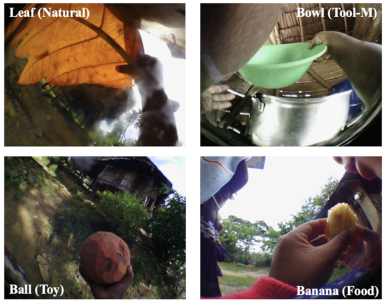
\includegraphics{figs/examples-fig-1} 

}

\caption[Example images with object and category labels]{Example images with object and category labels.}\label{fig:examples-fig}
\end{figure}
\end{CodeChunk}

\hypertarget{manual-annotation}{%
\subsection{Manual annotation}\label{manual-annotation}}

We annotated photos with IMCO (version 2.0, Casey, Fisher, Tice, \&
Casillas, 2022), an open-source Python application adapted for efficient
coding of photo streams. Annotators provided labels for the handled
object(s) present in each photo (e.g., ``twig'') and selected among
predefined categories to characterize each type of object (e.g.,
``natural object'') present. Categories included food, tools, toys,
immovable objects (e.g., furniture and housing structures), natural
objects, and miscellaneous synthetic objects (see Figure 1 for example
images and Table \ref{tab:top-objects} for example objects from each
category).

\hypertarget{data-preparation-and-reliability}{%
\subsection{Data preparation and
reliability}\label{data-preparation-and-reliability}}

Images were excluded if they were too dark, bright, blurry, or covered
for annotators to identify handled objects (128 images, 0.84\% of the
data set), if annotators were otherwise unsure about what objects were
being handled (592, or 3.89\%), if there was no handled object (25, or
0.16\%), or if the researcher was present (3, or 0.02\%). To avoid
unnecessary data loss, all excluded photos were checked by at least one
other annotator and re-included for analysis if objects were
identifiable. In total, 15232 images were deemed usable by annotators
(8556 for Rossel, 6656 for Tseltal).

XX\% of photo streams were double coded. Reliability annotations were
equally spread across sites and ages and included a total of XXXX
images. At the category level, annotators agreed on XX.X\% of decisions
(Rossel: XX.X\%, Tseltal: XX.X\%). At the object label level, annotators
agreed on XX.X\% of decisions (Rossel: XX.X\%, Tseltal: XX.X\%).

\begin{table}[!ht]
\centering
\scalebox{0.8}{
\begin{tabular}{lll}
  \hline
Object Category & Rossel & Tseltal \\ 
  \hline
Synthetic & shirt, woven basket, blanket & shirt, pants, shoe \\ 
  Food & betelnut, coconut, candy & bean, tortilla, soda \\ 
  Tool & knife, bowl, spoon & bowl, cup, bottle \\ 
  Toy & ball, book, swing & toy truck, book, ball \\ 
  Natural & stick, leaf, rock & stick, plant, tree \\ 
  Immovable & wall, stairs, veranda & chair, door, fence \\ 
   \hline
\end{tabular}
}
\caption{Non-study-related objects handled by the most children across categories and sites.} 
\label{tab:top-objects}
\end{table}

\hypertarget{results}{%
\section{Results}\label{results}}

\hypertarget{overall-frequency-statistics}{%
\subsection{Overall frequency
statistics}\label{overall-frequency-statistics}}

Children handled an average of 26.65 unique objects per day (median =
26, \emph{SD} = 15.65, range = 1--62), with no significant differences
across sites (\emph{M}\textsubscript{\emph{Rossel}} = 25.92,
\emph{M}\textsubscript{\emph{Tseltal}} = 27.46, \emph{W} = 661.5,
\emph{p} = 0.824). The distribution of handled objects was highly
right-skewed within and across children. Each child's distribution was
skewed such that a small group of objects were handled in a majority of
their images but most were handled for only short periods of time
(Figure 2). Across children, common objects followed a similar Zipfian
distribution: some objects were handled by many children, but most
objects were only handled by 1-2 children in each site (Rossel: 60.94\%,
Tseltal: 67.66\%).

\begin{CodeChunk}
\begin{figure}[h]

{\centering \includegraphics{figs/zipfian-objects-fig-1} 

}

\caption[Zipfian distribution of objects handled by each child across sites]{Zipfian distribution of objects handled by each child across sites. For each child, the top object was defined as the object appearing in the greatest number of images; thus, the identity of the top object does not match across all children.}\label{fig:zipfian-objects-fig}
\end{figure}
\end{CodeChunk}

Comparing across sites, 28.77\% of objects were present in both
communities, and several shared objects were among the most frequently
handled by children in both sites. In fact, among the top 25 most common
objects, 11 were shared across sites (Figure 3). Of note, the study
camera was the object handled by the most children in both sides
(Rossel: 69.2\%, Tseltal: 91.4\% of children). The camera and other
study-related objects (i.e., vest and privacy cover for the camera),
were retained in our analyses; however, inclusion of these items did not
qualitatively change any of the reported results.

\begin{CodeChunk}
\begin{figure*}[!ht]

{\centering \includegraphics{figs/top-objects-fig-1} 

}

\caption[Non-study-related objects handled at least once by the most children in each site]{Non-study-related objects handled at least once by the most children in each site. Filled bars represent objects that were among the top 25 for both sites.}\label{fig:top-objects-fig}
\end{figure*}
\end{CodeChunk}

\hypertarget{effects-of-object-category}{%
\subsection{Effects of object
category}\label{effects-of-object-category}}

The frequency of object categories was similarly divided across sites
(Figure 4A). The top objects for each category are shown in Table 1.
Children primarily handled miscellaneous synthetic objects (e.g., rope,
shirt, container, etc., \emph{M}\textsubscript{\emph{Rossel}} = 32.22\%,
\emph{M}\textsubscript{\emph{Tseltal}} = 36.9\% of handling) and food
(\emph{M}\textsubscript{\emph{Rossel}} = 28.32\%,
\emph{M}\textsubscript{\emph{Tseltal}} = 32.65\% of handling). For 56 of
74 children, their top category was either synthetic objects or food.
Two-tailed Wilcoxon tests revealed only one significant category-level
difference between sites: children's handling of large or immovable
objects (e.g., hammock, wall, stairs, etc.), where Rossel children
handled these objects more frequently than Tseltal children
(\emph{M}\textsubscript{\emph{Rossel}} = 10.29\%,
\emph{M}\textsubscript{\emph{Tseltal}} = 3.29\%, adjusted \emph{p} =
0.002, \emph{p}s for all other categories \textgreater{} 0.05), but
these objects were still the least frequently handled in both sites.

\begin{CodeChunk}
\begin{figure}[!h]

{\centering \includegraphics{figs/overall-stats-fig-1} 

}

\caption[(A) Overall frequency of handling by object category]{(A) Overall frequency of handling by object category. Points reflect percentages for individual children. (B) Count of unique objects handled per hour by object category. Points reflect means for individual children across all hours of recording.}\label{fig:overall-stats-fig}
\end{figure}
\end{CodeChunk}

During any given hour, children handled 6.44 objects from 3.14 different
categories, on average (median = 6 objects, \emph{SD} = 4.58, range =
1--28). To test for differences across sites and categories, we ran
individual linear mixed-effects models for each of the six object
categories, where objects belonging to the target category for a given
model were coded as 1, and objects belonging to other categories were
coded as 0. Models included fixed effects of site, category, and their
interaction as well as random intercepts for individual children. After
correcting for multiple comparisons, we found a significant main effect
of the synthetic object category (\(\beta\) = 1.06, \emph{SE} = 0.11,
\emph{t} = 9.79, \emph{p} \textless{} 0.001) along with a marginal
interaction between site and synthetic object category (\(\beta\) = 0.4,
\emph{SE} = 0.15, \emph{t} = 2.7, \emph{p} = 0.091) such that children
handled more unique synthetic objects per hour than other object
categories, and this effect was stronger for Tseltal children than for
Rossel children. Additionally, we found negative main effects for the
food (\(\beta\) = -0.47, \emph{SE} = 0.13, \emph{t} = -3.66, \emph{p} =
0.004), tool (\(\beta\) = -0.44, \emph{SE} = 0.14, \emph{t} = -3.19,
\emph{p} = 0.02) , and toy (\(\beta\) = -0.79, \emph{SE} = 0.18,
\emph{t} = -4.4, \emph{p} \textless{} 0.001) categories, meaning that
children handled fewer unique objects from these categories per hour
than other categories. Finally, a significant interaction between site
and the immovable object category revealed that Tseltal children handled
fewer unique immovable objects per hour than Rossel children. (\(\beta\)
= -0.9, \emph{SE} = 0.23, \emph{t} = -3.88, \emph{p} = 0.002; Figure
4B).

\hypertarget{effects-of-age}{%
\subsection{Effects of age}\label{effects-of-age}}

Children's overall rate of object handling increased significantly with
age (Figure 5A). That is, older children handled more unique objects per
hour (\(\beta\) = 0.1, \emph{SE} = 0.03, \emph{t} = 3.1, \emph{p} =
0.003). Additionally, with increasing age, children handled more objects
from different categories per hour (Figure 5B; \(\beta\) = 0.04,
\emph{SE} = 0.01, \emph{t} = 4.33, \emph{p} = 0). These effects were
consistent across sites; we found no main effects of site or
interactions between site and age (all \emph{p}s \textgreater{} 0.05).

To further explore developmental changes in the characteristics of
children's object handling, we measured transitions between different
objects and different object categories. We modeled the relative number
of transitions per hour (i.e., number of transitions divided by the
number of possible objects or categories for the hour) as a function of
age and site, plus their interaction. We found no overall age-related
increase in object transitions (\(\beta\) = , \emph{SE} = , \emph{t} = ,
\emph{p} = ). However, this analysis revealed a significant main effect
of site (\(\beta\) = -0.42, \emph{SE} = 0.13, \emph{t} = -3.11, \emph{p}
= 0.003) as well as a site-by-age interaction (\(\beta\) = 0.01,
\emph{SE} = 0, \emph{t} = 2.35, \emph{p} = 0.021) such that Tseltal
children made fewer transitions between objects per hour than Rossel
children but showed a steeper increase with age (Figure 5C). At the
category level, we found that, with age, children made significantly
more transitions between object categories per hour (\(\beta\) = 0.02,
\emph{SE} = 0.01, \emph{t} = 2.34, \emph{p} = 0.022), with no detectable
differences across sites (Figure 5D).

\begin{CodeChunk}
\begin{figure}[!ht]

{\centering \includegraphics{figs/age-effects-fig-1} 

}

\caption[(A) Unique objects and (B) object categories handled per hour as a function of age]{(A) Unique objects and (B) object categories handled per hour as a function of age. (C) Relative number of transitions between objects and (D) object categories per hour as a function of age. Points reflect raw hourly counts for each child, and lines reflect model predictions with shaded standard error regions.}\label{fig:age-effects-fig}
\end{figure}
\end{CodeChunk}

\hypertarget{discussion}{%
\section{Discussion}\label{discussion}}

{[}Overview para{]}

{[}Para on zipfian distributions and implications for word learning{]}:
Findings of skewed input are consistent with prior work describing
visual/object input (\textbf{clerkin2017real?};
\textbf{long2021characterizing?}) and language input
(\textbf{montag2018quantity?}). These Zipfian distributions can be
helpful for learning {[}(\textbf{carvalho2019rethinking?}); others{]}.
Overlap between kids can get us to start thinking about what some of the
earliest-learned object names are. BUT less overlap between kids (within
sites) than we see for US context (e.g., Herzberg, Fletcher, Schatz, \&
Tamis-LeMonda, 2021)

{[}Para on how we can also use these data to probe for time-of-day
consistencies and routinized activities{]}: Limitations of our current
coding of categories (e.g., mealtime tools and tools for
working/cleaning grouped together but perhaps mealtime tools are better
paired with food). Open question: are handled objects a good index for
activity context? (maybe some examples of why we think possibly yes, but
other examples to show why this would still be messy)

{[}Para on developmental change{]}. Broad composition of handled objects
was largely stable across age (consistent with
\textbf{long2021characterizing?} for visually present categories)

\hypertarget{references}{%
\section{References}\label{references}}

\setlength{\parindent}{-0.1in} 
\setlength{\leftskip}{0.125in}

\noindent

\hypertarget{refs}{}
\begin{CSLReferences}{1}{0}
\leavevmode\hypertarget{ref-adolph2010motor}{}%
Adolph, K. E., Karasik, L. B., \& Tamis-LeMonda, C. S. (2010). Motor
skill. In M. H. Bornstein (Ed.), \emph{Handbook of cultural
developmental science} (pp. 61--88). Psychology Press: New York, NY.

\leavevmode\hypertarget{ref-arnold2012life}{}%
Arnold, J. E., Graesch, A. P., Ochs, E., \& Ragazzini, E. (2012).
\emph{Life at home in the twenty-first century: 32 families open their
doors}. ISD LLC.

\leavevmode\hypertarget{ref-bergelson2019day}{}%
Bergelson, E., Amatuni, A., Dailey, S., Koorathota, S., \& Tor, S.
(2019). Day by day, hour by hour: Naturalistic language input to
infants. \emph{Developmental Science}, \emph{22}(1), e12715.

\leavevmode\hypertarget{ref-bergelson2017nature}{}%
Bergelson, E., \& Aslin, R. N. (2017). Nature and origins of the lexicon
in 6-mo-olds. \emph{Proceedings of the National Academy of Sciences},
\emph{114}(49), 12916--12921.

\leavevmode\hypertarget{ref-brownIPchildrearing}{}%
Brown, P., \& Casillas, M. (2021). \emph{Childrearing through social
interaction on {Rossel Island, PNG}}. (A. J. Fentiman \& M. Goody,
Eds.). New York, NY: Berghahn.

\leavevmode\hypertarget{ref-casey2022imco}{}%
Casey, K., Fisher, W., Tice, S. C., \& Casillas, M. (2022). ImCo: A
python tkinter application for coding lots of images (Version 2.0).
Retrieved from \url{https://github.com/kennedycasey/ImCo2}

\leavevmode\hypertarget{ref-casillas2020early}{}%
Casillas, M., Brown, P., \& Levinson, S. C. (2020). Early language
experience in a {Tseltal Mayan} village. \emph{Child Development},
\emph{91}(5), 1819--1835.

\leavevmode\hypertarget{ref-casillas2021early}{}%
Casillas, M., Brown, P., \& Levinson, S. C. (2021). Early language
experience in a papuan community. \emph{Journal of Child Language},
\emph{48}(4), 792--814.

\leavevmode\hypertarget{ref-casillasURdaylong}{}%
Casillas, M., \& Elliott, M. (2021). Cross-cultural differences in
children's object handling at home. PsyArXiv.
http://doi.org/\href{https://doi.org/10.31234/osf.io/43db8}{10.31234/osf.io/43db8}

\leavevmode\hypertarget{ref-fausey2016faces}{}%
Fausey, C. M., Jayaraman, S., \& Smith, L. B. (2016). From faces to
hands: Changing visual input in the first two years. \emph{Cognition},
\emph{152}, 101--107.

\leavevmode\hypertarget{ref-gaskins2000childrens}{}%
Gaskins, S. (2000). Children's daily activities in a {M}ayan village: A
culturally grounded description. \emph{Cross-Cultural Research},
\emph{34}(4), 375--389.

\leavevmode\hypertarget{ref-herzberg2021exuberant}{}%
Herzberg, O., Fletcher, K. K., Schatz, J. L., \& Tamis-LeMonda, C. S.
(2021). Infant exuberant object play at home: Immense amounts of
time-distributed, variable practice. \emph{Child Development},
\emph{XX}, 1--15.

\leavevmode\hypertarget{ref-jayaraman2017faces}{}%
Jayaraman, S., Fausey, C. M., \& Smith, L. B. (2017). Why are faces
denser in the visual experiences of younger than older infants?
\emph{Developmental Psychology}, \emph{53}(1), 38.

\leavevmode\hypertarget{ref-karasik2018not}{}%
Karasik, L. B., Schneider, J., Kuchirko, Y. A., \& Tamis-LeMonda, C. S.
(2018). Not so {WEIRD} object play in {T}ajikistan. Presentation to the
International Conference on Infant Studies, Philadelphia, PA.
http://doi.org/\href{https://doi.org/10.31234/osf.io/43db8}{10.31234/osf.io/43db8}

\leavevmode\hypertarget{ref-kretch2014crawling}{}%
Kretch, K. S., Franchak, J. M., \& Adolph, K. E. (2014). Crawling and
walking infants see the world differently. \emph{Child Development},
\emph{85}(4), 1503--1518.

\leavevmode\hypertarget{ref-laing2020babble}{}%
Laing, C., \& Bergelson, E. (2020). From babble to words: Infants' early
productions match words and objects in their environment.
\emph{Cognitive Psychology}, \emph{122}, 101308.

\leavevmode\hypertarget{ref-long2020detecting}{}%
Long, B., Kachergis, G., Agrawal, K., \& Frank, M. C. (2020).
\emph{Detecting social information in a dense database of infants'
natural visual experience}.

\leavevmode\hypertarget{ref-mcgillion2013supporting}{}%
McGillion, M. L., Herbert, J. S., Pine, J. M., Keren-Portnoy, T.,
Vihman, M. M., \& Matthews, D. E. (2013). Supporting early vocabulary
development: What sort of responsiveness matters? \emph{IEEE
Transactions on Autonomous Mental Development}, \emph{5}(3), 240--248.

\leavevmode\hypertarget{ref-sanchez2018detecting}{}%
Sanchez, A., Long, B., Kraus, A. M., \& Frank, M. C. (2018). Postural
developments modulate children's visual access to social information. In
\emph{Proceedings of the 40th annual conference of the cognitive science
society} (pp. 2412--2417).

\leavevmode\hypertarget{ref-super1976environmental}{}%
Super, C. M. (1976). Environmental effects on motor development: The
case of {`{A}frican infant precocity.'} \emph{Developmental Medicine \&
Child Neurology}, \emph{18}(5), 561--567.

\leavevmode\hypertarget{ref-yu2013joint}{}%
Yu, C., \& Smith, L. B. (2013). Joint attention without gaze following:
Human infants and their parents coordinate visual attention to objects
through eye-hand coordination. \emph{PloS One}, \emph{8}(11), e79659.

\leavevmode\hypertarget{ref-yurovsky2013statistical}{}%
Yurovsky, D., Smith, L. B., \& Yu, C. (2013). Statistical word learning
at scale: The baby's view is better. \emph{Developmental Science},
\emph{16}(6), 959--966.

\end{CSLReferences}

\bibliographystyle{apacite}


\end{document}
